\clearpage
\section{Backpropagation}

Dans cette section, on continue d'implémenter la \textit(Backpropagation) avec le calcul du gradient.
De plus, on entrainera le réseau de neurone à l'aide de la fonction d'optimisation avancée 
\textit{fmin\_cg} qui nous permet d'obtenir une fonction de coût $J(\theta)$ minimale. 


\subsection{Sigmoid gradient}

La formule du gradient du sigmoïde est obtenue avec la formule suivante.

\begin{equation}
    g'(z) = \frac{d}{dz}g(z) = g(z)(1 - g(z)) \qquad \qquad \text{avec} \quad \qquad \text{sigmoid}(z) = g(z) = \frac{1}{1 + e^{-z}}
\end{equation}

\noindent
\textbf{Implémentation}

\begin{figure}[!h]
    \begin{minted}[frame=lines, framesep=2mm, baselinestretch=1.2, fontsize=\footnotesize, linenos, breaklines=true]{python}
    def sigmoidGradient(z):

        g = sigmoid(z) * (1 - sigmoid(z))
        
        return g

    """return 
    Evaluating sigmoid gradient...
    Sigmoid gradient evaluated at [1 -0.5 0 0.5 1]:[0.19661193 0.23500371 0.25       0.23500371 0.19661193]
    (this value should be about 0.196612 0.235004 0.250000 0.235004 0.196612)       
    """
    \end{minted}   
    \captionof{listing}{\label{lst:sigmoidGradient}sigmoidGradient}
\end{figure}

\subsection{Random initialization}

Comme décrit dans le TP, il est important d'initialiser 
les paramètres de manière aléatoire pour casser la symétrie. On va donc appliquer la formule qui suit, 
de sorte à garder des paramètres petits pour rendre l'apprentissage plus efficace. 

\begin{equation}
    \epsilon_{\text{init}} = \frac{\sqrt{6}}{\sqrt{L_{\text{in}} + L_{\text{out}}}} \quad \text{avec} \quad L_{\text{in}} = S_l = 10 \quad \text{et} \quad L_{\text{out}} = S_{(l+1)} = 10+1
\end{equation}

\noindent
\textbf{Implémentation}

\begin{figure}[!h]
    \begin{minted}[frame=lines, framesep=2mm, baselinestretch=1.2, fontsize=\footnotesize, linenos, breaklines=true]{python}

    def randInitializeWeights(L_in, L_out):

        # Randomly initialize the weights to small values
        epsilon_init = 0.12
        W = np.random.rand(L_out, 1+L_in) * 2 * epsilon_init - epsilon_init

        return W
    \end{minted}   
    \captionof{listing}{\label{lst:randInitializeWeights}randInitializeWeights}
\end{figure}

\subsection{Backpropagation algorithm}

A partir de cette section, nous n'avons plus à coder puisque l'essentiel du code est déjà implémenté.
Nous allons donc synthétiser ce que nous avons compris de cet algorithme et des sections qui suivent
cette partie.

\begin{figure}[!h]
    \begin{center}
        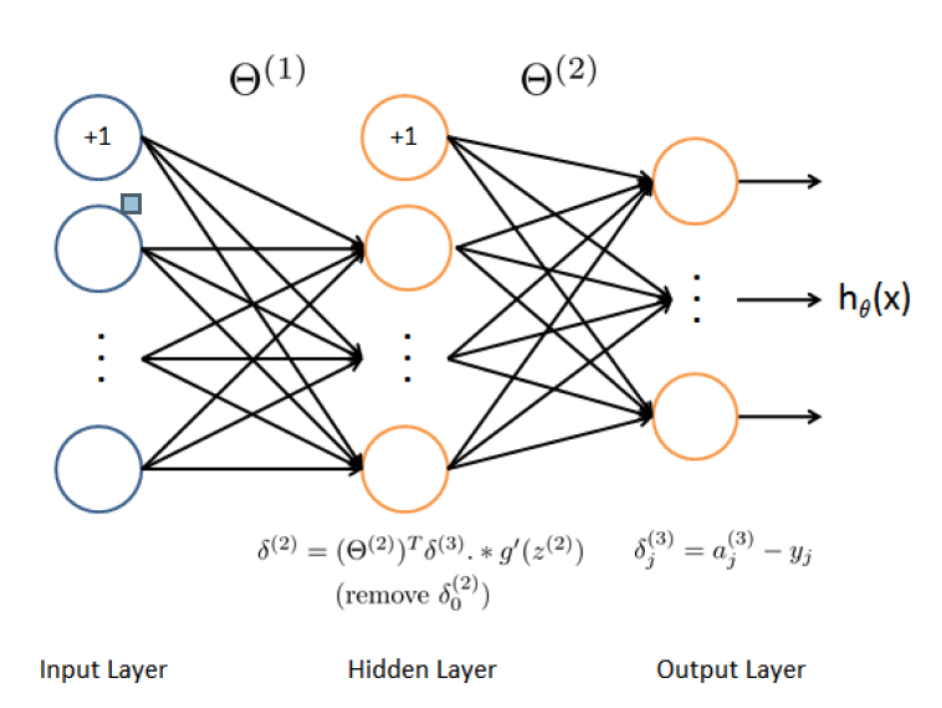
\includegraphics[width=0.75\textwidth]{./img/3.3.png}
        \caption{\label{fig:3.3}Backpropagagtion updates}  
    \end{center}
\end{figure}

Le principe décrit est le suivant, au démarrage, les calculs génèrent une propagation avant jusqu'à
la sortie et obtenir l'erreur $h_{\theta}((x))_k$. Le but principal est de réussir à évaluer quels noeuds
va le plus influencer l'erreur de sortie. Pour obtenir l'erreur il suffit de faire la différence entre la
sortie du réseau de neurone et les valeurs ciblées de Y. //

Pour arriver à un résultat correcte qui minimise l'erreur, il faut suivre quatre étapes pour chaque échantillons
d'entrainement donnés. Ainsi, à chaque itération, en s'entrainant à chaque boucle, le réseau devient plus
performant. 

\begin{enumerate}
    \item Propagation avant (Forward Pass)
    \item Calcul de l'erreur de la couche de sortie
    \item Calcul de l'erreur des couches cachées
    \item Addition des gradients pour chaque échantillon
    \item Normalisation des gradients
\end{enumerate}

Une fois la dernière étape du dernier échantillon passé, les gradients moyens sont utilisés pour définir
et surtout mettre à jour les poids du réseau afin de minimiser l'impacte des noeuds qui augmentent l'erreur. 

\subsection{Gradient checking}

Dans cette section, l'objectif est de vérifier chacun de nos gradients préalablement calculés. Le code fourni
dans \textit(computeNumericalGradient.py) fonctionne de telle manière à venir tronquer les valeurs de ${\theta}$. 
A chaque itération, une composante de ${\theta}$ est perturbée par ${\epsilon}$ puis le coût est réévalué. Pour finir,
la formule du gradient numérique est utilisée pour évaluer chaque nouvelles compsantes du gradient numérique. 
Cette fonction retourne \textit{numgrad} qui servira de comparateur avec les valeurs calculées par notre algorithme
de rétropropagation. Plus les écarts sont minimes, mieux l'algorithme se comporte et est bien entraîné.

\vspace{0.4cm}
\noindent
\textbf{Résultat du gradient checking}

\begin{figure}[!h]
    \begin{minted}[frame=lines, framesep=2mm, baselinestretch=1.2, fontsize=\footnotesize, linenos, breaklines=true]{python}
    """return 
    Checking Backpropagation... 
    [[-9.27825235e-03 -9.27825236e-03]
    [ 8.89911959e-03  8.89911960e-03]
    [-8.36010761e-03 -8.36010762e-03]
    [ 7.62813550e-03  7.62813551e-03]
    [-6.74798369e-03 -6.74798370e-03]
    [-3.04978709e-06 -3.04978914e-06]
    [ 1.42869450e-05  1.42869443e-05]
    [ 4.65597186e-02  4.65597186e-02]]
    The above two columns you get should be very similar.
    (Left-Your Numerical Gradient, Right-Analytical Gradient)

    If your backpropagation implementation is correct, then
    the relative difference will be small (less than 1e-9). 

    Relative Difference: 2.4768e-11 
    """
    \end{minted}   
    \captionof{listing}{\label{lst:computeNumericalGradients}Compute Numerical Gradient}
\end{figure}

\noindent
Le résultat obtenu est satisfaisant puisque l'écart est inférieur à la différence relative annoncée. 

\clearpage

\subsection{Regularized Neural Networks}

De la même manière que pour les autres TP, on vient régulariser le gradient. La rétropropagation nous a 
permis de calculer les gradients, le but ici est d'appliquer les formules données dans le sujet pour 
régulariser le réseau de neurone. 

\begin{align}
    \frac{\partial J(\Theta)}{\partial \Theta_{ij}^{(l)}} = \frac{1}{m} \Delta_{ij}^{(l)} + \frac{\lambda}{m} \Theta_{ij}^{(l)} \quad \text{pour} \quad  J = 0   \\
    \frac{\partial J(\Theta)}{\partial \Theta_{ij}^{(l)}} = \frac{1}{m} \Delta_{ij}^{(l)} + \frac{\lambda}{m} \Theta_{ij}^{(l)} \quad \text{pour} \quad  J >= 1
\end{align}

\vspace{0.4cm}
\noindent
\textbf{Résultat du Regularized gradient}

\begin{figure}[!h]
    \begin{minted}[frame=lines, framesep=2mm, baselinestretch=1.2, fontsize=\footnotesize, linenos, breaklines=true]{python}
    """return 
    Checking Backpropagation (w/ Regularization) ... 
    [[-9.27825235e-03 -9.27825236e-03]
    [ 8.89911959e-03  8.89911960e-03]
    [-8.36010761e-03 -8.36010762e-03]
    [ 7.62813550e-03  7.62813551e-03]
    [-6.74798369e-03 -6.74798370e-03]
    [-1.67679797e-02 -1.67679797e-02]
    [ 3.94334829e-02  3.94334829e-02]
    [ 1.50048382e-03  1.50048382e-03]]
    The above two columns you get should be very similar.
    (Left-Your Numerical Gradient, Right-Analytical Gradient)


    If your backpropagation implementation is correct, then
    the relative difference will be small (less than 1e-9). 

    Relative Difference: 2.34399e-11
    """
    \end{minted}   
    \captionof{listing}{\label{lst:RegularizedGradient}Regularized Gradient}
\end{figure}

\noindent
Le résultat obtenu est satisfaisant puisque l'écart est inférieur à la différence relative annoncée. 

\subsection{Learning parameters using fmin}

Avec la fonction \texttt{fmin\_cg}, le système apprends un bon ensemble de paramètres. Ce qui permet de vérifier
si l'entraînement de notre réseau de neurone est correcte par rapport à l'esemble d'entraînement. 

\vspace{0.4cm}
\noindent
\textbf{Résultat}

\begin{figure}[!h]
    \begin{minted}[frame=lines, framesep=2mm, baselinestretch=1.2, fontsize=\footnotesize, linenos, breaklines=true]{python}
    """return 
    Visualizing Neural Network... 
    Training Set Accuracy: 96.000000
    """
    \end{minted}   
    \captionof{listing}{\label{lst:fmin_cg}\texttt{fmin\_cg} function}
\end{figure}


